% ----------------------------------------------------------
% LaTeX Article *******************************
% -----------------------------------------------------------
% Preamble

% Define the type of document you are writing
\documentclass[11pt]{article}		

% declare the packages you need..
\usepackage{amsmath, amsfonts, amsthm, amssymb}  % these let you use all the fancy math fonts, symbols etc.
\usepackage{color, fullpage, hyperref}  % you can add colour with the color package
\usepackage{graphicx}

% Set the indent of new paragraphs to 0 so that paragraphs are not indented.
\setlength{\parindent}{0pt}


\title{MAT B42 Cheatsheet}
\author{Jiaming Lu}

% End Preamble

\begin{document}
\maketitle
\newpage   % creates a page break

\tableofcontents % this makes a table of contents of all my sections

\newpage


\section{Vector Valued Function}
\subsection{Vector Field}
$\mathbf{F} : A \subset \mathbb{R}^n\to \mathbb{R}^n$

\subsection{Flow Lines}
If $\mathbf{F}$ is a vector field, a flow line for $\mathbf{F}$ is a path $c(t)$ such that
\[c'(t) = \mathbf{F}(c(t))\]

\section{Divergence and Curl}
\subsection{Divergence}
\[ {\rm div} \ \mathbf{F} = \nabla \cdot \mathbf{F}\]

\subsection{Curl}
\[ {\rm curl} \ \mathbf{F} = \nabla \times \mathbf{F}\]

\subsection{Properties of div and curl}
\textbf{Curl of a Gradient}
\[\nabla \times (\nabla f) = \mathbf{0}\]
\begin{proof}
    \begin{eqnarray*}
      \nabla \times (\nabla f) &=&  
      \begin{vmatrix} \mathbf{i} & \mathbf{j} & \mathbf{k} \\
        \frac{\partial}{\partial{x}} & \frac{\partial}{\partial{y}} & \frac{\partial}{\partial{z}}\\
        \frac{\partial f}{\partial{x}} & \frac{\partial f}{\partial{y}} & \frac{\partial f}{\partial{z}} \end{vmatrix}\\
        &=& \left(\frac{\partial^{2} f}{\partial y \partial z}-\frac{\partial^{2} f}{\partial z \partial y}\right) \mathbf{i}+\left(\frac{\partial^{2} f}{\partial z \partial x}-\frac{\partial^{2} f}{\partial x \partial z}\right) \mathbf{j}+\left(\frac{\partial^{2} f}{\partial x \partial y}-\frac{\partial^{2} f}{\partial y \partial x}\right) \mathbf{k}\\
        &=& \mathbf{0}
    \end{eqnarray*}
\end{proof}
\textbf{Divergence of a Curl}
\[\nabla \cdot(\nabla \times \mathrm{F})=0\]
\textbf{Properties of Vector Field}
\[\begin{aligned}
    \mathbf{F}=\nabla f & \Rightarrow  \operatorname{curl} \mathbf{F}=\mathbf{0} \\
    \mathbf{F}=\nabla \times \mathbf{G} & \Rightarrow \operatorname{div} \mathbf{F}=0
\end{aligned}\]
\begin{proof}
    Let
    \[\begin{aligned}
        G_{1}&=\int_{0}^{z} F_{2}(x, y, t) d t-\int_{0}^{y} F_{3}(x, t, 0) d t ,~
        G_{2}&=-\int_{0}^{z} F_{1}(x, y, t) d t,~
        G_3 &= 0
    \end{aligned}\]
\end{proof}
\newpage
\textbf{Basic Identities of Vector Analysis}
\begin{enumerate}
    \item $\nabla(f+g)=\nabla f+\nabla g$
    \item $\nabla(c f)=c \nabla f$, for a constant $c$
    \item $\nabla(f g)=f \nabla g+g \nabla f$
    \item $\nabla(f / g)=(g \nabla f-f \nabla g) / g^{2}$, at points $\mathrm{x}$ where $g(\mathrm{x}) \neq 0$
    \item $\operatorname{div}(\mathbf{F}+\mathbf{G})=\operatorname{div} \mathbf{F}+\operatorname{div} \mathbf{G}$
    \item $\operatorname{curl}(\mathbf{F}+\mathbf{G})=\operatorname{curl} \mathbf{F}+\operatorname{curl} \mathbf{G}$
    \item $\operatorname{div}(f \mathbf{F})=f \operatorname{div} \mathbf{F}+\mathbf{F} \cdot \nabla f$
    \item $\operatorname{div}(\mathbf{F} \times \mathbf{G})=\mathbf{G} \cdot \operatorname{curl} \mathbf{F}-\mathbf{F} \cdot \operatorname{curl} \mathbf{G}$
    \item {\color{red} $\operatorname{div}$ curl $\mathbf{F}=\mathbf{0}$}
    \item $\operatorname{curl}(f \mathbf{F})=f \operatorname{curl} \mathbf{F}+\nabla f \times \mathbf{F}$
    \item {\color{red}$\operatorname{curl} \nabla f=\mathbf{0}$}
    \item $\nabla^{2}(f g)=f \nabla^{2} g+g \nabla^{2} f+2(\nabla f \cdot \nabla g)$
    \item $\operatorname{div}(\nabla f \times \nabla g)=\mathbf{0}$
    \item $\operatorname{div}(f \nabla g-g \nabla f)=f \nabla^{2} g-g \nabla^{2} f$
\end{enumerate}

\newpage

\section{Integrals Over Path and Surfaces}
\subsection{The Path Integrals}
\[\int_{\mathbf{c}} f d s= \int_{a}^{b} f(\mathbf{c}(t))\left\|\mathbf{c}^{\prime}(t)\right\| d t\]

\subsection{Line Integral}
\[\int_{\mathbf{c}} \mathbf{F} \cdot d \mathbf{s}=\int_{a}^{b} \mathbf{F}(\mathbf{c}(t)) \cdot \mathbf{c}^{\prime}(t) dt\]
\\
\textbf{Theorem 1}
Change of Parametrization for Line Integrals \\ 
Let $\mathbf{F}$ be a vector field continuous on the $C^{1}$ path $\mathbf{c}:\left[a_{1}, b_{1}\right] \rightarrow \mathbb{R}^{3}$, and let $\mathbf{p}:[a, b] \rightarrow \mathbb{R}^{3}$ be a re-parametrization of $\mathbf{c}$. If $\mathbf{p}$ is orientation-preserving, then
$$
\int_{\mathbf{p}} \mathbf{F} \cdot d \mathbf{s}=\int_{\mathbf{c}} \mathbf{F} \cdot d \mathbf{s}
$$
and if $\mathbf{p}$ is orientation-reversing, then
$$
\int_{\mathbf{p}} \mathbf{F} \cdot d \mathbf{s}=-\int_{\mathbf{c}} \mathbf{F} \cdot d\mathbf{s}
$$
\\
\textbf{Theorem 3} Line Integrals of Gradient Vector Fields \\
Suppose $f: \mathbb{R}^{3} \rightarrow \mathbb{R}$ is of class $C^{1}$ and that $c:[a, b] \rightarrow \mathbb{R}^{3}$ is a piecewise $C^{1}$ path. Then
$$
\int_{c} \nabla f \cdot d \mathbf{s}=f(\mathbf{c}(b))-f(\mathbf{c}(a))
$$
\\
\textbf{Line Integrals Over Curves with Opposite Orientations}\\
 Let $C^{-}$be the same curve as $C$, but with the opposite orientation. Then
$$
\int_{C} \mathbf{F} \cdot d \mathbf{s}=-\int_{C^{-}} \mathbf{F} \cdot d \mathbf{s}
$$
\\
\textbf{Line Integrals Over Curves Consisting of Several Components}\\ 
Let $C$ be an oriented curve such that $C=C_{1}+C_{2}+\cdots+C_{k}$. So we have:
$$
\int_{C} \mathbf{F} \cdot d \mathbf{s}=\int_{C_{1}} \mathbf{F} \cdot d \mathbf{s}+\int_{C_{2}} \mathbf{F} \cdot d \mathbf{s}+\cdots+\int_{C_{k}} \mathbf{F} \cdot d \mathbf{s}
$$
\newpage
\subsection{Area of a Surface}
\textbf{Definition} Regular Surface\\
A surface is regular iff. $\mathbf{T}_{u} \times \mathbf{T}_{v} \ne \mathbf{0}$\\\\
\textbf{Area of a Parametrized Surface}
\[A(S)=\iint_{D}\left\|\mathbf{T}_{u} \times \mathbf{T}_{v}\right\| d u dv\]
\\
If $\mathbf{\Phi} = (u,v,g(u,v))$,
\[A(S)=\iint_{D}\left(\sqrt{\left(\frac{\partial g}{\partial x}\right)^{2}+\left(\frac{\partial g}{\partial y}\right)^{2}+1}\right) d A\]
\begin{proof}
    \[\mathbf{T}_{u}=\mathbf{i}+\frac{\partial g}{\partial u} \mathbf{k}, \quad \mathbf{T}_{v}=\mathbf{j}+\frac{\partial g}{\partial v} \mathbf{k}
    \]\[
    \mathbf{T}_{u} \times \mathbf{T}_{v}=-\frac{\partial g}{\partial u} \mathbf{i}-\frac{\partial g}{\partial v} \mathbf{j}+\mathbf{k}=-\frac{\partial g}{\partial x} \mathbf{i}-\frac{\partial g}{\partial y} \mathbf{j}+\mathbf{k}
    \]
    \[||\mathbf{T}_{u} \times \mathbf{T}_{v}|| = \sqrt{\left(\frac{\partial g}{\partial x}\right)^{2}+\left(\frac{\partial g}{\partial y}\right)^{2}+1}\]
\end{proof}

\textbf{Surface of Revolution}\\
The lateral surface area generated by revolving the graph of a function $y = f (x)$ about the x-axis is given by
\[A=2 \pi \int_{a}^{b}\left(|f(x)| \sqrt{1+\left[f^{\prime}(x)\right]^{2}}\right) d x\]
\begin{proof}
    Let $S: \mathbf{\Phi}(u,v) = (u, f(u) \cos v, f(u) \sin v)$, so we have:
    \[\frac{\partial(x, y)}{\partial(u, v)}=-f(u) \sin v, \quad \frac{\partial(y, z)}{\partial(u, v)}=f(u) f^{\prime}(u), \quad \frac{\partial(x, z)}{\partial(u, v)}=f(u) \cos v\]
    \[\begin{aligned}
        A(S) &=\iint_{D} \sqrt{\left[\frac{\partial(x, y)}{\partial(u, v)}\right]^{2}+\left[\frac{\partial(y, z)}{\partial(u, v)}\right]^{2}+\left[\frac{\partial(x, z)}{\partial(u, v)}\right]^{2}} d u d v \\
        &=\iint_{D} \sqrt{[f(u)]^{2} \sin ^{2} v+[f(u)]^{2}\left[f^{\prime}(u)\right]^{2}+[f(u)]^{2} \cos ^{2} v} d u d v \\
        &=\iint_{D}|f(u)| \sqrt{1+\left[f^{\prime}(u)\right]^{2}} d u d v \\
        &=\int_{a}^{b} \int_{0}^{2 \pi}|f(u)| \sqrt{1+\left[f^{\prime}(u)\right]^{2}} d v d u \\
        &=2 \pi \int_{a}^{b}|f(u)| \sqrt{1+\left[f^{\prime}(u)\right]^{2}} d u
        \end{aligned}\]
\end{proof}

\subsection{Surface Integral}
\begin{enumerate}
    \item Parametrized Surface: $\boldsymbol{\Phi}(u, v)$
    \begin{itemize}
        \item[a.] Integral of a scalar function $f$ :
        $$
        \iint_{S} f d S=\iint_{D} f(\boldsymbol{\Phi}(u, v))\left\|\mathbf{T}_{u} \times \mathbf{T}_{v}\right\| d u d v
        $$
        \item[b.] Scalar surface element:
        $$
        d S=\left\|\mathbf{T}_{u} \times \mathbf{T}_{v}\right\| d u d v
        $$

        \item[c.] Integral of a vector field $\mathbf{F}$ :
        $$
        \iint_{S} \mathbf{F} \cdot d \mathbf{S}=\iint_{D} \mathbf{F} \cdot\left(\mathbf{T}_{u} \times \mathbf{T}_{v}\right) d u d v
        $$
        \item[d.] Vector surface element:
        $$
        d \mathbf{S}=\left(\mathbf{T}_{u} \times \mathbf{T}_{v}\right) d u d v=\mathbf{n} d S
        $$
    \end{itemize}

    \item Graph: $z=g(x, y)$
    \begin{enumerate}
        \item[a.] Integral of a scalar function $f$ :
        $$
        \iint_{S} f d S=\iint_{D} \frac{f(x, y, g(x, y))}{\cos \theta} d x d y=\iint_{D} \frac{f(x, y, g(x, y))}{\mathbf{n\cdot k}} d x d y
        $$
        \item[b.] Scalar surface element:
        $$
        d S=\frac{d x d y}{\cos \theta}=\sqrt{\left(\frac{\partial g}{\partial x}\right)^{2}+\left(\frac{\partial g}{\partial y}\right)^{2}+1} d x d y
        $$
        where $\cos \theta=\mathbf{n} \cdot \mathbf{k}$, and $\mathbf{n}$ is a unit normal vector to the surface.
        \item[c.] Integral of a vector field $\mathrm{F}$ :
        $$
        \iint_{S} \mathbf{F} \cdot d \mathbf{S}=\iint_{D}\left(-F_{1} \frac{\partial g}{\partial x}-F_{2} \frac{\partial g}{\partial y}+F_{3}\right) d x d y
        $$
        \item[d.] Vector surface element:
        $$
        d \mathbf{S}=\mathbf{n} \cdot d S=\left(-\frac{\partial g}{\partial x} \mathbf{i}-\frac{\partial g}{\partial y} \mathbf{j}+\mathbf{k}\right) d x d y
        $$
    \end{enumerate} 
    \item Sphere: $x^{2}+y^{2}+z^{2}=R^{2}$
    \begin{enumerate}
        \item[a.] Scalar surface element:
        $$
        d S=R^{2} \sin \phi d \phi d \theta
        $$
        \item[b.] Vector surface element:
        $$
        d \mathbf{S}=(x \mathbf{i}+y \mathbf{j}+z \mathbf{k}) R \sin \phi d \phi d \theta=\mathrm{r} R \sin \phi d \phi d \theta=\mathrm{n} R^{2} \sin \phi d \phi d \theta
        $$
    \end{enumerate}
       
\end{enumerate}

\section{Classic Theorems of Vector Calculus}
\subsection{Green's Theorem}
\textbf{Green's Theorem} \\
If $F = P\mathbf{i}+Q\mathbf{j}$, and $C^+$ is a simple closed curve(orients anticlockwisly about the region $D$):
\[\int_{C^{+}} P d x+Q d y=\iint_{D}\left(\frac{\partial Q}{\partial x}-\frac{\partial P}{\partial y}\right) d x d y\]
\begin{proof}
    \textbf{Lemma1} 
    \[ \iint_{D} \frac{\partial P}{\partial y}(x, y) d x d y = -\int_{C^{+}} P dx\]
    \begin{figure}[htbp]
        \centering
        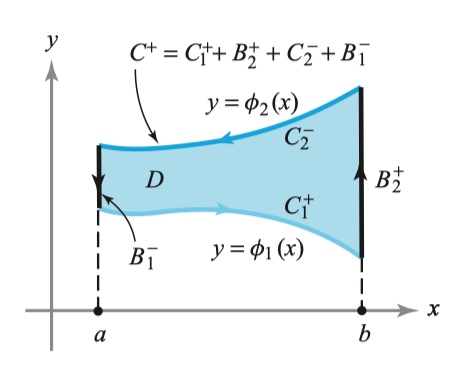
\includegraphics[width=6.5cm]{Lemma 1.jpg}
    \end{figure}\\
    \textsc{Proof}
    \[\begin{aligned}
        \iint_{D} \frac{\partial P}{\partial y}(x, y) d x d y &=\int_{a}^{b} \int_{\phi_{1}(x)}^{\phi_{2}(x)} \frac{\partial P}{\partial y}(x, y) d y d x \\
        &=\int_{a}^{b}\left[P\left(x, \phi_{2}(x)\right)-P\left(x, \phi_{1}(x)\right)\right] dx \\
        &= -(\int_{C_{1}^{+}} P d x - \int_{C_{2}^{+}} P d x)\\
        &= -(\int_{C_{1}^{+}} P d x + 0 + \int_{C_{2}^{-}} P d x + 0)\\
        &= -(\int_{C_{1}^{+}} P d x+\int_{B_{2}^{+}} P d x+\int_{C_{2}^{-}} P d x+\int_{B_{1}^{-}} P d x)\\
        &= -\int_{C^{+}} P dx
    \end{aligned}\]
    \begin{flushright}QED.\end{flushright}
    \newpage
    \textbf{Lemma 2}
    \[\int_{C^{+}} Q d y=\iint_{D} \frac{\partial Q}{\partial x} d x d y\]
    \textsc{Proof}
    \[\begin{aligned}
        \iint_{D} \frac{\partial Q}{\partial x} d x d y &=\int_{c}^{d} \int_{\psi_{1}(y)}^{\psi_{2}(y)} \frac{\partial Q}{\partial x} d x d y=\int_{c}^{d}\left[Q\left(\psi_{2}(y), y\right)-Q\left(\psi_{1}(y), y\right)\right] d y \\
        &=\int_{C_{2}^{+}} Q d y-\int_{C_{1}^{+}} Q d y=\int_{C_{2}^{+}} Q d y+\int_{C_{1}^{-}} Q d y=\int_{C^{+}} Q d y
    \end{aligned}\]
    \begin{flushright}QED.\end{flushright}
    By combining Lemma 1 and Lemma 2, we thus proved Green's Theorem.
\end{proof}
\textsc{Note:}\\
For non-simple region, we can divides the region into sub-regions and apply Green's Theorem.
\begin{figure}[htbp]
    \centering
    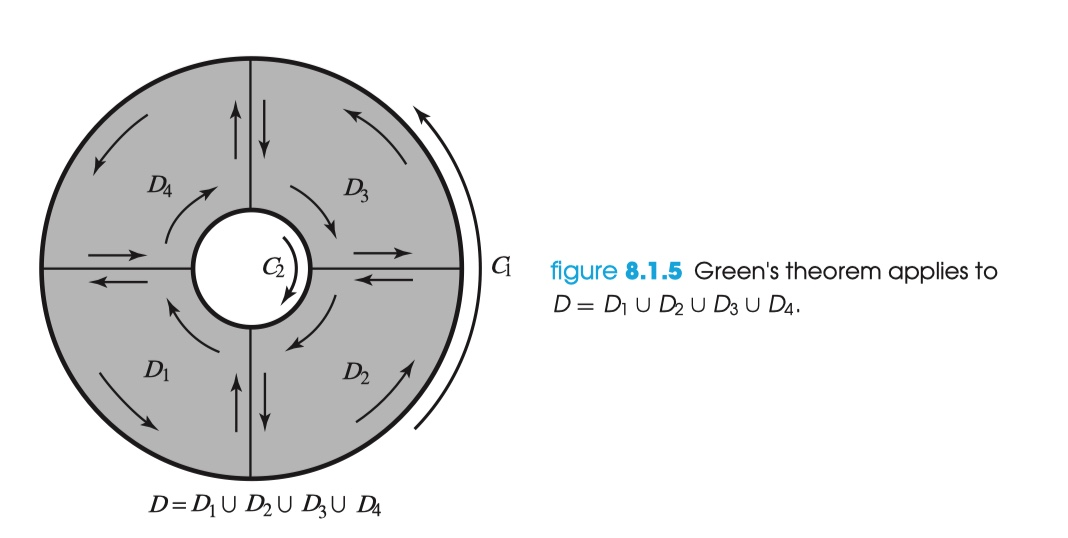
\includegraphics[width=10cm]{GGT.jpg}
\end{figure}\\
\textbf{Area of a Region}
\\ Can be proved by Green's Theorem
\[A=\frac{1}{2} \int_{\partial D} x d y-y d x\]

\newpage

\subsection{Stoke's Theorem}
\textbf{Theorem 6} Stoke's Theorem\\
If $S$ is a $C^2$ surface parametrized by $\mathbf{\Phi}(u,v) = (u,v,f(u,v))$, and $\mathbf{F}$ is a $C^1$ vector field on $S$, $\partial S$ is the boundary of $S$, we have
\[\iint_{S} \operatorname{curl} \mathbf{F} \cdot d \mathbf{S}=\iint_{S}(\nabla \times \mathbf{F}) \cdot d \mathbf{S}=\int_{\partial S} \mathbf{F} \cdot d \mathbf{s}\]
\\
\begin{proof}
    \[
        \iint_{S} \operatorname{curl} \mathbf{F} \cdot d \mathbf{S}= \iint_{D}\left[\left(\frac{\partial F_{3}}{\partial y}-\frac{\partial F_{2}}{\partial z}\right)\left(-\frac{\partial z}{\partial x}\right)+\left(\frac{\partial F_{1}}{\partial z}-\frac{\partial F_{3}}{\partial x}\right)\left(-\frac{\partial z}{\partial y}\right)+\left(\frac{\partial F_{2}}{\partial x}-\frac{\partial F_{1}}{\partial y}\right)\right] d A
    \]
    And,
    \[
    \begin{aligned}
        \int_{\partial S} \mathbf{F} \cdot d \mathbf{s}
        &=\int_{a}^{b}\left(F_{1} \frac{d x}{d t}+F_{2} \frac{d y}{d t}+F_{3} \frac{d z}{d t}\right) d t\\ 
        &=\int_{a}^{b}\left[\left(F_{1}+F_{3} \frac{\partial z}{\partial x}\right) \frac{d x}{d t}+\left(F_{2}+F_{3} \frac{\partial z}{\partial y}\right) \frac{d y}{d t}\right] d t \\
        &=\int_{\mathbf{c}}\left(F_{1}+F_{3} \frac{\partial z}{\partial x}\right) d x+\left(F_{2}+F_{3} \frac{\partial z}{\partial y}\right) d y \\
        &=\int_{\partial D}\left(F_{1}+F_{3} \frac{\partial z}{\partial x}\right) d x+\left(F_{2}+F_{3} \frac{\partial z}{\partial y}\right) d y .
    \end{aligned}
    \]
    By applying Green's Theorem, we have:
    \[
    \begin{aligned}
        \int_{\partial S} \mathbf{F} \cdot d \mathbf{s}&=\iint_{D}\left[\frac{\partial\left(F_{2}+F_{3} \partial z / \partial y\right)}{\partial x}-\frac{\partial\left(F_{1}+F_{3} \partial z / \partial x\right)}{\partial y}\right] d A\\
        &= \iint_{D}{\left[\left(\frac{\partial F_{2}}{\partial x}+\frac{\partial F_{2}}{\partial z} \frac{\partial z}{\partial x}+\frac{\partial F_{3}}{\partial x} \frac{\partial z}{\partial y}+\frac{\partial F_{3}}{\partial z} \frac{\partial z}{\partial x} \frac{\partial z}{\partial y}+F_{3} \frac{\partial^{2} z}{\partial x \partial y}\right)\right.} \\
        &-\left.\left(\frac{\partial F_{1}}{\partial y}+\frac{\partial F_{1}}{\partial z} \frac{\partial z}{\partial y}+\frac{\partial F_{3}}{\partial y} \frac{\partial z}{\partial x}+\frac{\partial F_{3}}{\partial z} \frac{\partial z}{\partial y} \frac{\partial z}{\partial x}+F_{3} \frac{\partial^{2} z}{\partial y \partial x}\right)\right] d A\\
        &= \iint_{D}\left[\left(\frac{\partial F_{3}}{\partial y}-\frac{\partial F_{2}}{\partial z}\right)\left(-\frac{\partial z}{\partial x}\right)+\left(\frac{\partial F_{1}}{\partial z}-\frac{\partial F_{3}}{\partial x}\right)\left(-\frac{\partial z}{\partial y}\right)+\left(\frac{\partial F_{2}}{\partial x}-\frac{\partial F_{1}}{\partial y}\right)\right] d A\\
        &=\iint_{S} \operatorname{curl} \mathbf{F} \cdot d \mathbf{S}
    \end{aligned}
    \]
\end{proof}

\newpage

\subsection{Conservative Fields}
\textbf{Theorem 7} Conservative Fields\\
Statements below are equivalent:
\begin{enumerate}
    \item[(i)] For any oriented simple closed curve $C, \int_{C} \mathbf{F} \cdot d \mathbf{s}=0$.
    \item[(ii)] For any two oriented simple curves $C_{1}$ and $C_{2}$ that have the same endpoints,
    $$
    \int_{C_{1}} \mathbf{F} \cdot d \mathbf{s}=\int_{C_{2}} \mathrm{~F} \cdot d \mathbf{s}
    $$
    \item[(iii)] $\exists f ~ s.t. ~\mathbf{F}=\nabla f$ 
    \\(and if $\mathbf{F}$ has one or more exceptional points where it fails to be defined, $f$ is also undefined there).
    \item[(iv)] $\nabla \times \mathbf{F}=\mathbf{0}$.
    \\ 
\end{enumerate}


\begin{proof}
    In order to prove the theorem, we establish following chain of implication:
    \[(i) \rightarrow (ii) \rightarrow (iii) \rightarrow (iv) \rightarrow (i)\]


    Proof of $(i) \rightarrow (ii)$:\\
    Let $\mathbf{c}=\mathbf{c_1}-\mathbf{c_2}$. By $(i)$:
    \[\int_{\mathbf{c}} \mathbf{F} \cdot d \mathbf{s}=\int_{\mathbf{c}_{1}} \mathbf{F} \cdot d \mathbf{s}-\int_{\mathbf{c}_{2}} \mathbf{F} \cdot d \mathbf{s}=0\]
    \[\leftrightarrow \int_{C_{1}} \mathbf{F} \cdot d \mathbf{s}=\int_{C_{2}} \mathbf{F} \cdot d \mathbf{s}\]
    \begin{flushright}QED.\end{flushright}
    

    Proof of $(ii) \rightarrow (iii)$:\\
    From $(ii)$, we know that $\mathbf{F}$ is path independent, so we can set up different path to complete the proof. Here's a example for proving $\frac{\partial f}{\partial z} = F_3$\\
    Choose $C$ is a simple curve with the path (0, 0, 0) to (x, 0, 0) to (x, y, 0) to (x, y, z)\\
    Define, $f = \int_{0}^{x} F_{1}(t, 0,0) d t+\int_{0}^{y} F_{2}(x, t, 0) d t+\int_{0}^{z} F_{3}(x, y, t) dt$. Therefore, $\frac{\partial f}{\partial z} = F_3$. 
    \begin{flushright}QED.\end{flushright}

    Proof of $(iii) \rightarrow (iv)$:\\
    See in section2.3\\
    

    Proof of $(iv) \rightarrow (i)$:
    \[\int_{C} \mathbf{F} \cdot d \mathbf{s}=\int_{\mathbf{c}} \mathbf{F} \cdot d \mathbf{s}=\iint_{S}(\nabla \times \mathbf{F}) \cdot \mathbf{n} d S=\iint_{S}\mathbf{0} \cdot \mathbf{n} d S=0\]
    \begin{flushright}QED.\end{flushright}
\end{proof}

\newpage

\textbf{Corollary 1} \\
$\mathrm{~F}$ is a $C^{1}$ vector field on $\mathbb{R}^{2}$ of the form $P \mathbf{i}+Q \mathrm{j}$ that satisfies $\partial P / \partial y=\partial Q / \partial x$, then $\mathrm{F}=\nabla f$ for some $f$ on $\mathbb{R}^{2}$.\\

\textbf{Theorem 8} \\
If $\mathrm{F}$ is a $C^{1}$ vector field on all of $\mathbb{R}^{3}$ with $\operatorname{div} \mathbf{F}=0$, then there exists a $C^{1}$ vector field $\mathbf{G}$ with $\mathbf{F}=\operatorname{curl} \mathbf{G}$.
\begin{proof}
    Define $\mathbf{G}=G_{1} \mathbf{i}+G_{2} \mathbf{j}+G_{3} \mathbf{k}$ by
    $$
    \begin{aligned}
    &G_{1}(x, y, z)=\int_{0}^{z} F_{2}(x, y, t) d t-\int_{0}^{y} F_{3}(x, t, 0) d t \\
    &G_{2}(x, y, z)=-\int_{0}^{z} F_{1}(x, y, t) d t\\
    &G_3(x,y,z) = 0
    \end{aligned}
    $$
    Therefore, $\nabla \times \mathbf{G} = (F_1,F_2,F_3) = \mathbf{F}$
\end{proof}


\subsection{Gauss Theorem}
\textbf{Theorem 9} Gauss’ Divergence Theorem
\[\iiint_{W}({\rm div} ~\mathbf{F}) d V=\iiint_{W}(\nabla \cdot \mathbf{F}) d V=\iint_{\partial W} \mathbf{F} \cdot d \mathbf{S}\]

\textbf{Theorem 10} Gauss’ Law
\[\iint_{\partial M} \frac{\mathbf{r} \cdot \mathbf{n}}{||\mathbf{r}||^{3}} d S= \begin{cases}4 \pi & \text { if }(0,0,0) \in M \\ 0 & \text { if }(0,0,0) \notin M\end{cases}\]

\begin{proof}
If $(0,0,0)\notin M$. Then $\frac{\mathbf{r}}{r^3}$ is $C^1$. So by Gauss' Theorem,
$$\iint_{\partial W} \frac{\mathbf{r} \cdot \mathbf{n}}{\|\mathbf{r}\|^{3}}dS=\iiint_{W} \operatorname{div}\left(\frac{\mathbf{r}}{\|\mathbf{r}\|^{3}}\right) d V=\iiint_{W} 0 d V=0$$

If $(0,0,0)\in M$. Because $M$ is no longer $C^1$, so we needs a unit ball $N$ centered $(0,0,0)$ of radius $\epsilon > 0$ to exclude the origin. Therefore, 

$$
\begin{aligned}
    \iint_{\partial N} \mathbf{F} \cdot \mathbf{n} d S &=\iint_{\partial N} \frac{(x, y, z) \cdot\left(\frac{x}{\epsilon}, \frac{y}{\epsilon}, \frac{z}{\epsilon}\right)}{\left(x^{2}+y^{2}+z^{2}\right)^{3 / 2}} d S \\
    &=\frac{1}{\epsilon} \iint_{\partial N} \frac{x^{2}+y^{2}+z^{2}}{\left(x^{2}+y^{2}+z^{2}\right)^{3 / 2}} d S=\frac{1}{\epsilon} \iint_{\partial N} \frac{1}{\sqrt{x^{2}+y^{2}+z^{2}}} d S \\
    &=\frac{1}{\epsilon} \iint_{\partial N} \frac{1}{\sqrt{\epsilon^{2}}} d S=\frac{1}{\epsilon^{2}} \iint_{\partial N} d S=\frac{1}{\epsilon^{2}}\left(4 \pi \epsilon^{2}\right)=4 \pi
    \end{aligned}
$$
As the result,
$$\iint_{\partial W} \frac{\mathbf{r} \cdot \mathbf{n}}{\|\mathbf{r}\|^{3}}=\iint_{\partial N} \mathbf{F} \cdot \mathbf{n} d S+\iint_{\partial W \setminus \partial N} \mathbf{F} \cdot \mathbf{n} d S=4\pi$$

\end{proof}

\newpage

\subsection{Differential form}
\textbf{Definition}
Differentiation $d: \bigwedge^k \to \bigwedge^{k+1}$, with properties:
\begin{enumerate}
    \item If  $f \in \bigwedge^{0}$, then  $df=\frac{\partial f}{\partial x} d x+\frac{\partial f}{\partial y} d y+\frac{\partial f}{\partial x} d z$
    \item $d\left(\omega_{1}+\omega_{2}\right)=d \omega_{1}+d \omega_{2}$
    \item If  $\omega \in \bigwedge^{k}$, then $d(\omega \wedge \eta)=(d \omega) \wedge \eta+(-1)^{k} \omega \wedge(d \eta) $
    \item As a linear map  $d^{2}=0 $
\end{enumerate}
\textbf{Definition}
Wedge $\wedge: \bigwedge^{k} \times \bigwedge^{\ell} \rightarrow \bigwedge^{k+\ell}$, with porperties:
\begin{enumerate}
    \item $0 \wedge \omega=0$
    \item $\left(f \omega_{1}+\omega_{2}\right) \wedge \eta=(f)\left(\omega_{1} \wedge \eta\right)+\omega_{2} \wedge \eta $
    \item $\omega \wedge \eta=(-1)^{k \ell} \eta \wedge \omega $
    \item $\omega_{1} \wedge\left(\omega_{2} \wedge \omega_{3}\right)=\left(\omega_{1} \wedge \omega_{2}\right) \wedge \omega_{3}$
    \item If  $f$  is a $0$ -form then  $f \wedge \omega=f \omega$
\end{enumerate}

\textbf{Definition}

A form is closed $d\omega = 0$ and it is exact if $\omega= d\eta$.

\textbf{Theorem}
    
Exact implies closed.
$\\$

\textbf{Theorem 11} Green's Theorem

$D$ is an elementary region, with $\partial D$ given the counterclockwise orientation. Suppose $\omega = P(x,y)dx + Q(x,y)dy$ is a 1-form on some open set $K$ in $\mathbb{R}^3$ that contains $D$. Then
$$\int_{\partial D} \omega=\iint_{D} d \omega$$

\textbf{Theorem 12} Stokes' Theorem

$S$ is an oriented surface on $\mathbb{R}^3$ with boundary $\partial S$.Suppose $\omega$ is a 1-form on some open set $K$ that contains $S$. Then
$$\int_{\partial S} \omega=\iint_{S} d \omega$$

\textbf{Theorem 13} Gauss' Theorem

Let $W \subset \mathbb{R}^3$ be an elementary region with $\partial W$ given the outward orientation. If $\eta$ is a 2-form on some region $K$ containing $W$, then
$$\iint_{\partial W} \eta=\iiint_{W} d \eta$$

\newpage

\section{Fourier expansion and PDEs}
\subsection{Fourier polynomial}
\textbf{Definition}
$$\langle f(x), g(x)\rangle=\int_{-\pi}^{\pi} f(x) g(x) d x$$
This is a symmetric bilinear inner product. The corresponding norm is $L^2$-norm:
$$\|f\|_{2}^{2}=\int_{-\pi}^{\pi}[f(x)]^{2} d x$$


\textbf{Lemma}

For a inner product space $(V,\langle \cdot,\cdot \rangle)$. If $\{\vec{v}_0,...,\vec{v}_n\}$ is an orthogonal set of vectors and $\vec{x}\in {\rm span}\{\vec{v}_0,...,\vec{v}_n\}$, then:
$$\vec{x}=\frac{\left\langle\vec{x}, \vec{v}_{0}\right\rangle}{\left\langle\vec{v}_{0}, \vec{v}_{0}\right\rangle} \vec{v}_{0}+\frac{\left\langle\vec{x}, \vec{v}_{1}\right\rangle}{\left\langle\vec{v}_{1}, \vec{v}_{1}\right\rangle} \vec{v}_{1}+\cdots+\frac{\left\langle\vec{x}, \vec{v}_{n}\right\rangle}{\left\langle\vec{v}_{n}, \vec{v}_{n}\right\rangle} \vec{v}_{n}$$


\textbf{Definition}

The Fourier basis for $L^2([-\pi,\pi])$ is $$\{1\}\cup \bigcup_{n \in \mathbb{N}}\{\cos (n x), \sin (n x)\}$$

\textbf{Definition}

The $n$-th Fourier polynomial $F_n(x)$ of $f(x)$ has the form:
$$F_{n}(x)=a_{0}+\sum_{k=1}^{n} a_{k} \cos (k x)+\sum_{k=1}^{n} b_{k} \sin (k x)$$
where:
$$a_{0}=\frac{1}{2 \pi} \int_{-\pi}^{\pi} f(x) d x \quad a_{k}=\frac{1}{\pi} \int_{-\pi}^{\pi} f(x) \cos (k x) d x \quad b_{k}=\frac{1}{\pi} \int_{-\pi}^{\pi} f(x) \sin (k x) d x$$

\begin{proof}
    $$
    a_0=\frac{\langle 1,f \rangle}{\langle 1,1\rangle }\quad 
    a_k=\frac{\langle \cos(kx),f \rangle}{\langle\cos(kx),\cos(kx)\rangle}\quad 
    b_k=\frac{\langle \sin(kx),f \rangle}{\langle\sin(kx),\sin(kx)\rangle}
    $$
    as you should verify
\end{proof}


\textbf{Definition}

The energy of $f(x)$ is:
$$E=\frac{1}{\pi} \int_{-\pi}^{\pi}(f(x))^{2} d x$$
Alternatively, $E=\frac{1}{\pi} ||f ||_{2}^{2}$

\newpage

\subsection{Partial differential equations}
\textbf{Wave Equation}

Wave equations has the format
$$u_{tt} = c^2u_{xx}$$

It has solution 
$$u(x, t)=\sum_{n=1}^{\infty} \sin \left(\frac{n \pi x}{l}\right)\left(A_{n} \cos \left(\frac{n \pi c t}{l}\right)+B_{n} \sin \left(\frac{n \pi c t}{l}\right)\right)$$

Where 
$$A_{n}=\frac{2}{l} \int_{0}^{l} \phi(x) \sin \left(\frac{n \pi x}{l}\right)dx,~ B_{n}=\frac{2}{n \pi c} \int_{0}^{l} \psi(x) \sin \left(\frac{n \pi x}{l}\right)dx\\$$


\textbf{Heat equation}

Heat equations has the format
$$u_t = ku_{xx}$$

It has solution
$$u(x, t)=\sum_{n=0}^{\infty} A_{n} \cos \left(\frac{n \pi x}{l}\right) e^{-\left(\frac{n \pi}{l}\right)^{2} k t}$$

Where
$$A_{0}=\frac{1}{l} \int_{0}^{l} \phi(x)dx,~A_{m}=\frac{2}{l} \int_{0}^{l} \phi(x) \cos \left(\frac{m \pi x}{l}\right)dx,\quad m\neq 0$$


\end{document}
